\section{Auswertung}
\label{sec:Auswertung}

\subsection{Einstellung des Selektivverstärkers}
In Tabelle \ref{taba} sind die Frequenzen $\nu$ und die jeweils gemessenen Ausgangspannungen $U_\text{A}$ 
bei einer Eingangsspannung von $U_\text{E} = \SI{100}{\milli\volt}$ eingetragen. 
In Abb. \ref{plota} sind diese Werte gegeneinander aufgetragen.

\begin{table}\caption{Die Länge der Zylinder und die Spannung mit den jeweiligen Zeitenpunkten der Ausschläge.}
\label{taba}
\centering
\sisetup{round-mode = places, round-precision=2, round-integer-to-decimal=true}
\begin{tabular}{S[]S[]S[]S[]S[]} 
\toprule
{$l/ \si{\milli\meter}$} & {$U_1/ \si{\volt}$} & {$t_1/ \si{\micro\second}$} & {$U_2/ \si{\volt}$} & {$t_2/ \si{\micro\second}$}\\
\midrule
120.8 & 1.29 & 0.6 & 0.17 & 88.7\\
102.3 & 1.27 & 0.5 & 0.2 & 76.5\\
80.5 & 1.33 & 0.6 & 0.76 & 59.8\\
40.4 & 1.33 & 0.5 & 1.34 & 30.2\\
31.1 & 1.29 & 0.5 & 1.37 & 23.8\\
\bottomrule
\end{tabular}\end{table}

% Plot einfügen 
\begin{figure}
    \centering
    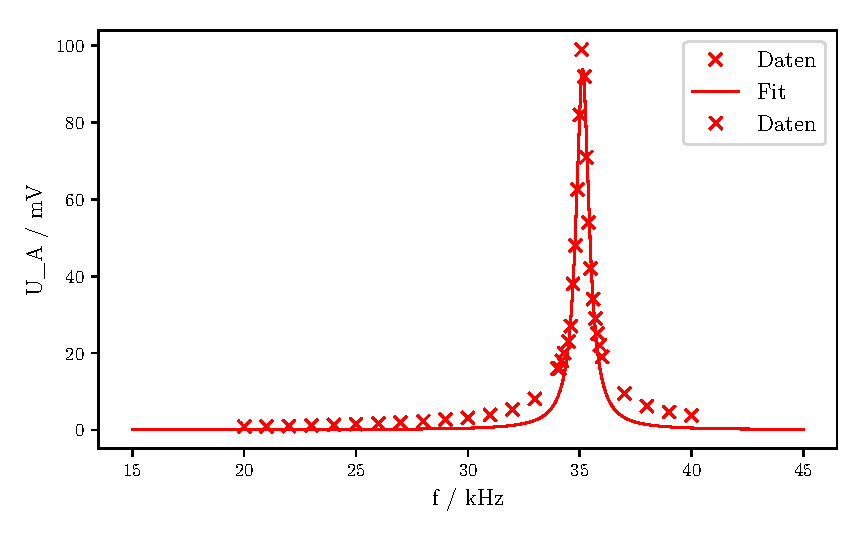
\includegraphics[width=15cm, height=8cm]{build/plota.pdf} %
    \caption{Die Filterkurve des Selektivverstärkers. Das Verhältnis der Ein- und Ausgangspannung
    ist gegen die Frequenz aufgetragen.}
    \label{plota}
\end{figure}

\noindent Aus der Tabelle lassen sich der Wert $\nu_0$ und die beiden Werte $\nu_\text{-}$ und $\nu_\text{+}$ ablesen. 
Diese ergeben sich zu 
\begin{align*} 
 \nu_0 &= \SI{<++>}{\kilo\hertz} \\
 \nu_{-} &= \SI{<++>}{\kilo\hertz} \\
 \nu_{+} &= \SI{<++>}{\kilo\hertz}. 
\end{align*}

\noindent Daraus lässt sich mit Gleichung \eqref{guete} erkennen, dass die Güte den Wert 
\begin{align*} 
    G_\text{exp} = \num{<++>}
\end{align*}
hat. 

\noindent Der gegebene Wert für $G$ liegt bei 
\begin{align*} 
    G = \num{100}.
\end{align*}


\subsection{Theoriewerte für Suszeptibilität} 
Für die verschiedenen Stoffe haben sich aufgrund der verschiedenen Elemente und Zusammensetzungen auch verschiedene 
Werte für die Suszeptibilität ergeben. 
Die Werte, die zur Berechnung nötig waren, sind ...
Für den Stoff $<++>$ ergibt sich die Rechnung folgendermaßen: 

\begin{equation*}
    <++>.
\end{equation*} 

\noindent Die anderen drei Werte lassen sich analog ermitteln. 
In Tab. \ref{tab1} befinden sich die Werte für $L$, $S$ und $J$. Daneben stehen jeweils die Werte, die sich für 
die Suszeptibilität $\chi$ ergeben. 

\begin{table}\caption{Der maximale Drehimpuls $L$, der Gesamtspin $S$ und der Gesamtdrehimpuls $J$ ergeben sich zum Landé-Faktor $g_\text{J}$ für die vier verschiedenen Elemente.}
\label{tab1}
\centering
\sisetup{round-mode = places, round-precision=2, round-integer-to-decimal=true}
\begin{tabular}{S[]S[]S[]S[]} 
\toprule
{$L$} & {$S$} & {$J$} & {$g_\text{J}$}\\
\midrule
5.0 & 1.0 & 4.0 & 0.8\\
0.0 & 3.5 & 3.5 & 2.0\\
6.0 & 1.5 & 4.5 & 0.7272727272727273\\
5.0 & 2.5 & 7.5 & 1.3333333333333333\\
\bottomrule
\end{tabular}\end{table} %falsche Tabelle


\subsection{Suszeptibilität mittels Spannungsverhältnis}
Die Werte für die Suszeptibilität, die mittels Gleichung \eqref{eqn:chiexp1} ergeben sich für die jeweiligen Stoffe 
zu folgenden Werten 

\begin{align*} 
   \chi_\text{C_6 O_{12} Pr_2} &= \num{<++>}\\
   \chi_\text{Nd_2 O_3} &= \num{<++>}\\
   \chi_\text{Gd_2 O_3} &= \num{<++>}\\
   \chi_\text{Dy_2 O_3} &= \num{<++>}.
\end{align*}


\subsection{Suszeptibilität mittels Widerstandsverhältnis}
Mit Gleichung \eqref{eqn:chiexp2} wird die Suszeptibilität der Proben bestimmt.
Es ergeben sich die Werte

\begin{align*} 
   \chi_\text{C_6 O_{12} Pr_2} &= \num{<++>}\\
   \chi_\text{Nd_2 O_3} &= \num{<++>}\\
   \chi_\text{Gd_2 O_3} &= \num{<++>}\\
   \chi_\text{Dy_2 O_3} &= \num{<++>}.
\end{align*}

